\documentclass[10pt]{article}
\usepackage[margin=0.7in]{geometry}
\usepackage{graphicx}
\usepackage{longtable}
\usepackage{array}
\usepackage{hyperref}
\hypersetup{colorlinks=true,linkcolor=blue,urlcolor=blue}
\setlength{\parindent}{0pt}
\setlength{\parskip}{6pt}
\begin{document}
\title{Optical Reference Downloader and Lumileds Cage Holder Report}
\date{Generated 2026-06-26T06:09:43.559960+00:00}
\maketitle
\section{Purpose}
This report documents the reusable downloader workflow and the current quick-design reference set for a Lumileds PCB holder that shares 30 mm cage geometry with Hengyang and Thorlabs optical parts.
\section{Reusable Downloader}
\begin{verbatim}
python3 cad/tools/optical_reference_downloader.py hengyang
python3 cad/tools/optical_reference_downloader.py hengyang --only gkm-010-polarizer-waveplate-holders
python3 cad/tools/optical_reference_downloader.py thorlabs --preset common-30mm-cage
python3 cad/tools/optical_reference_downloader.py thorlabs SM1L10 CP02T --asset-group Step --asset-group "CAD PDF"
python3 cad/tools/optical_reference_downloader.py report --compile
\end{verbatim}
\section{Lumileds Holder Geometry}
\begin{longtable}{p{0.47\linewidth}p{0.38\linewidth}}
\textbf{Parameter} & \textbf{Value} \\ \hline
body\_width\_mm & 40.0 \\
body\_height\_mm & 41.5 \\
body\_thickness\_mm & 11.0 \\
cage\_rod\_pitch\_mm & 30.0 \\
cage\_rod\_clearance\_diameter\_mm & 6.35 \\
rod\_boss\_diameter\_mm & 9.6 \\
light\_aperture\_diameter\_mm & 9.6 \\
pcb\_outer\_diameter\_mm & 24.0 \\
pcb\_pocket\_diameter\_mm & 24.7 \\
pcb\_pocket\_depth\_mm & 2.05 \\
pcb\_thickness\_mm & 1.6 \\
pcb\_mount\_pattern\_mm & 12.0 \\
pcb\_mount\_hole\_diameter\_mm & 2.35 \\
bottom\_post\_mount\_hole\_diameter\_mm & 4.2 \\
\end{longtable}
Reference family: Hengyang Optics 30 mm cage components\\
Primary reference: GT-090101\\
Print note: Cage and PCB pockets include practical print clearance; tune after test print.
\begin{figure}[h]
\centering
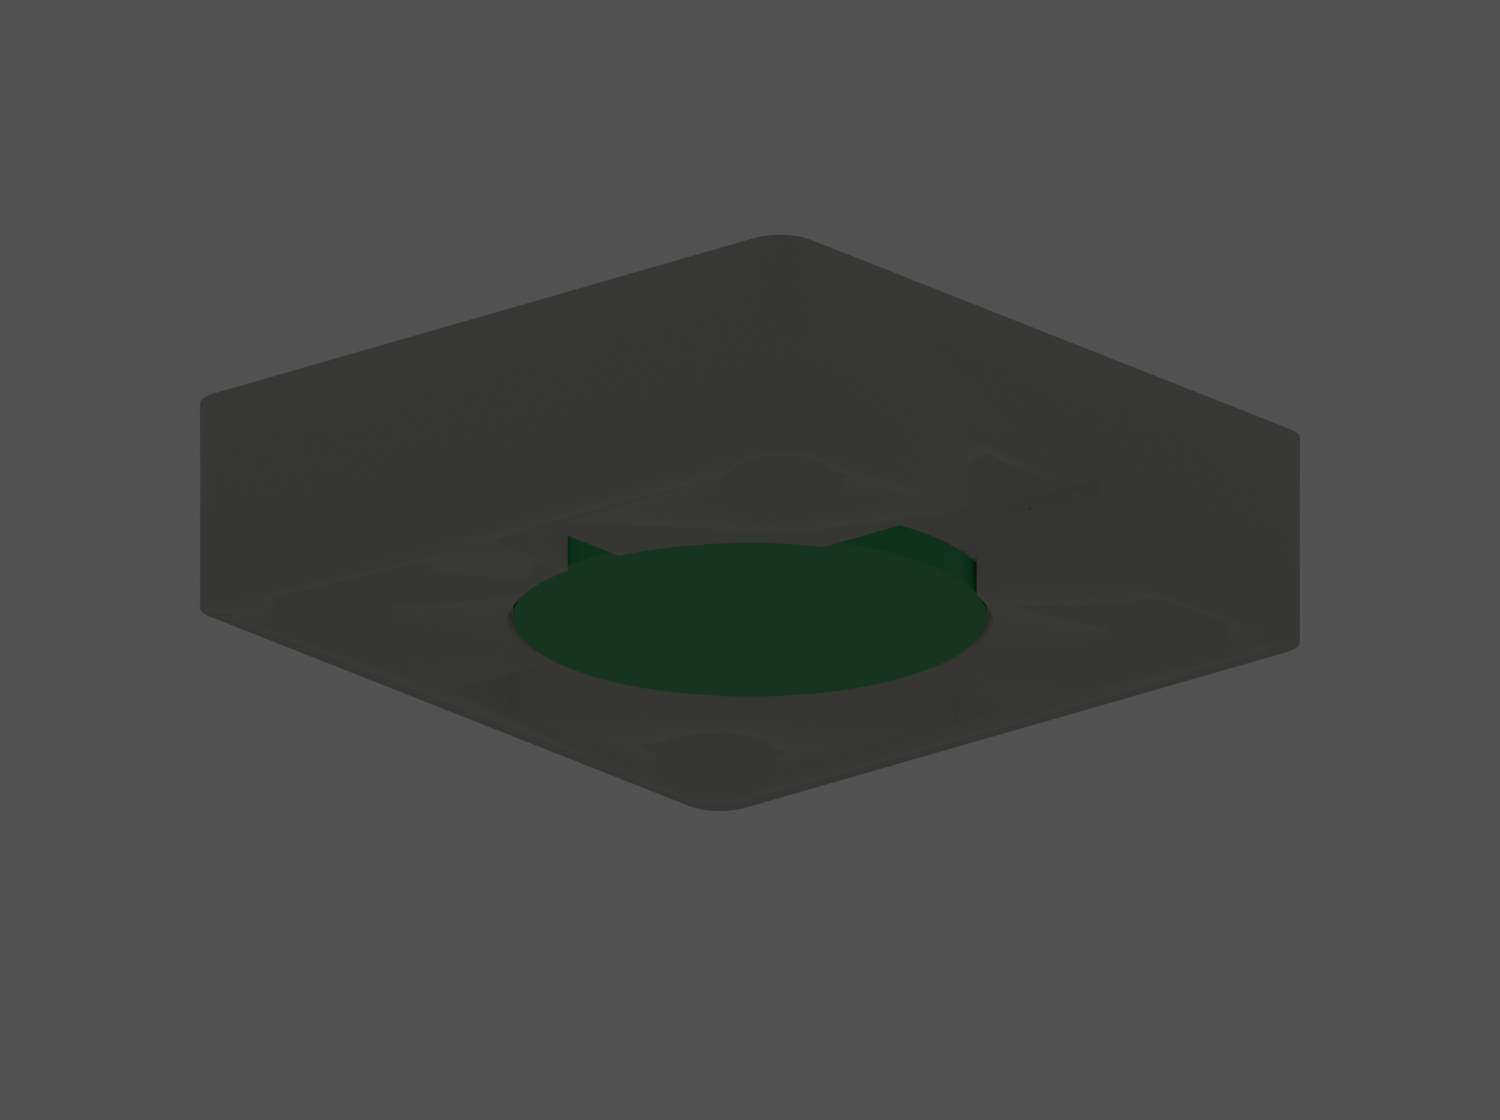
\includegraphics[width=0.72\linewidth]{../../designs/lumileds_hengyang_30mm_cage_holder/artifacts/lumileds_hengyang_30mm_cage_holder_render.png}
\caption{Lumileds holder inspection render.}
\end{figure}
\begin{figure}[h]
\centering
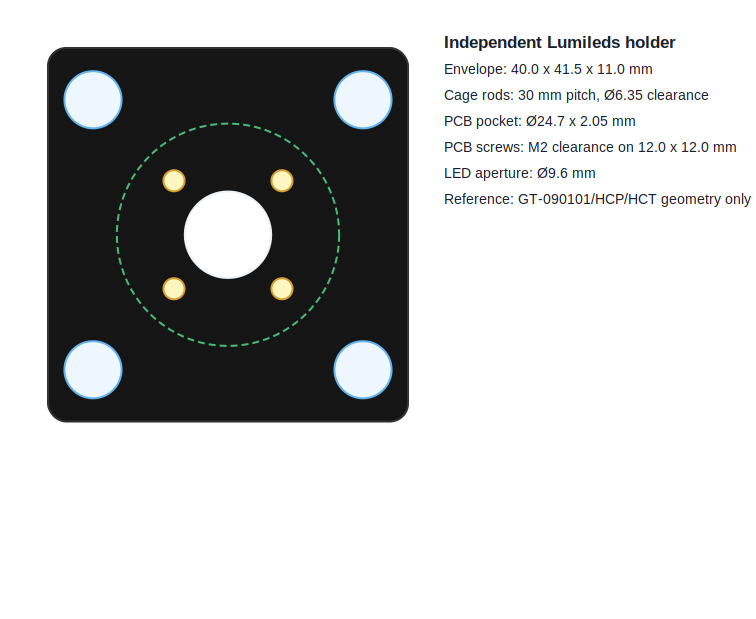
\includegraphics[width=0.72\linewidth]{../../designs/lumileds_hengyang_30mm_cage_holder/artifacts/lumileds_hengyang_30mm_cage_holder_dimension_sketch.png}
\caption{Dimension sketch for the holder.}
\end{figure}
\clearpage
\section{Hengyang Reference Set}
The Hengyang downloader captures category pages, API JSON, item JSON, drawings, STEP/STP files, and product images.
Manifest: \texttt{cad/references/hengyang-optics/manifest.json}
\begin{longtable}{p{0.18\linewidth}p{0.34\linewidth}p{0.36\linewidth}}
\textbf{Model} & \textbf{Category folder} & \textbf{Local files} \\ \hline
GT-090101 & gt-090101-waveplate-polarizer & drawing-pdf:1, item-json:1, model-stp:1, product-image:1 \\
HCP-22 & hcp-22-23-24-lens-cage-plates & drawing-pdf:1, item-json:1, model-step:1, product-image:1 \\
HCP23 & hcp-22-23-24-lens-cage-plates & drawing-pdf:1, item-json:1, model-step:1, product-image:1 \\
HCP24 & hcp-22-23-24-lens-cage-plates & drawing-pdf:1, item-json:1, model-step:1, product-image:1 \\
HCP-0801 & hcp-08-quick-lens-holders & drawing-pdf:1, item-json:1, model-step:1, product-image:1 \\
HCP-0804 & hcp-08-quick-lens-holders & drawing-pdf:1, item-json:1, model-step:1, product-image:1 \\
HCP-0805 & hcp-08-quick-lens-holders & drawing-pdf:1, item-json:1, model-stp:1, product-image:1 \\
GT-080303 & gt-0803-precision-lens-holders & drawing-pdf:1, item-json:1, model-stp:1, product-image:1 \\
GT-080304 & gt-0803-precision-lens-holders & drawing-pdf:1, item-json:1, model-stp:1, product-image:1 \\
HC-05 & hcm-3-beam-splitter-cube & drawing-pdf:1, item-json:1, model-stp:1, product-image:1 \\
HC-10 & hcm-3-beam-splitter-cube & drawing-pdf:1, item-json:1, model-stp:1, product-image:1 \\
HC-12.7 & hcm-3-beam-splitter-cube & drawing-pdf:1, item-json:1, model-stp:1, product-image:1 \\
HC-20 & hcm-3-beam-splitter-cube & drawing-pdf:1, item-json:1, model-stp:1, product-image:1 \\
HCM-3 & hcm-3-beam-splitter-cube & drawing-pdf:1, item-json:1, model-stp:1, product-image:1 \\
HCM-3C & hcm-3-flat-optic-45deg & drawing-pdf:1, item-json:1, model-stp:1, product-image:1 \\
HCM-3R & hcm-3-flat-optic-45deg & drawing-pdf:1, item-json:1, model-stp:1, product-image:1 \\
HCM-3B3C & hcm-3-flat-optic-45deg & drawing-pdf:1, item-json:1, model-stp:1, product-image:1 \\
HCM-3B4C & hcm-3-flat-optic-45deg & drawing-pdf:1, item-json:1, model-stp:1, product-image:1 \\
HKCB1PM & hkcb1pm-right-angle-mirror-holder & drawing-pdf:1, item-json:1, model-stp:1, product-image:1 \\
GKM-0101 & gkm-010-polarizer-waveplate-holders & drawing-pdf:1, item-json:1, model-step:1, product-image:1 \\
GKM-0102 & gkm-010-polarizer-waveplate-holders & drawing-pdf:1, item-json:1, model-step:1, product-image:1 \\
GKM-0103 & gkm-010-polarizer-waveplate-holders & drawing-pdf:1, item-json:1, model-step:1, product-image:1 \\
GKM-0104 & gkm-010-polarizer-waveplate-holders & drawing-pdf:1, item-json:1, model-step:1, product-image:1 \\
HCT-150 & hct-6mm-cage-rods & drawing-pdf:1, item-json:1, product-image:1 \\
HCT-150-P4 & hct-6mm-cage-rods & drawing-pdf:1, item-json:1, product-image:1 \\
HCT-150-P8 & hct-6mm-cage-rods & drawing-pdf:1, item-json:1, product-image:1 \\
HCT-010 & hct-6mm-cage-rods & drawing-pdf:1, item-json:1, model-step:1, product-image:1 \\
HCT-010-P4 & hct-6mm-cage-rods & drawing-pdf:1, item-json:1, model-step:1, product-image:1 \\
HCT-010-P8 & hct-6mm-cage-rods & drawing-pdf:1, item-json:1, model-step:1, product-image:1 \\
\end{longtable}
\section{Thorlabs Reference Set}
The Thorlabs downloader queries public product metadata and stores selected CAD assets by part number.
Manifest: \texttt{cad/references/thorlabs-optics/manifest.json}
\begin{longtable}{p{0.16\linewidth}p{0.42\linewidth}p{0.30\linewidth}}
\textbf{Part} & \textbf{Name} & \textbf{Local files} \\ \hline
C4W & C4W & CAD DXF:1, CAD PDF:1, Step:1, product-image:1, product-json:1 \\
CP02T & CP02T & CAD DXF:1, CAD PDF:1, Step:1, product-image:1, product-json:1 \\
ER1 & ER1 & CAD DXF:1, CAD PDF:1, Step:1, product-image:1, product-json:1 \\
ER2 & ER2 & CAD DXF:1, CAD PDF:1, Step:1, product-image:1, product-json:1 \\
KCB1 & KCB1 & CAD DXF:1, CAD PDF:1, Step:1, product-image:1, product-json:1 \\
KM100 & KM100 & CAD DXF:1, CAD PDF:1, Step:1, product-image:1, product-json:1 \\
LCP02 & LCP02 & CAD DXF:1, CAD PDF:1, Step:1, product-image:1, product-json:1 \\
SM1L10 & SM1L10 & CAD DXF:1, CAD PDF:1, Step:1, product-image:1, product-json:1 \\
\end{longtable}
\section{Measured STEP Bounds}
STEP bounds are approximate imported bounding boxes, useful for fast layout planning before detailed inspection.
\begin{longtable}{p{0.58\linewidth}p{0.10\linewidth}p{0.10\linewidth}p{0.10\linewidth}}
\textbf{STEP file} & \textbf{X mm} & \textbf{Y mm} & \textbf{Z mm} \\ \hline
cad/references/hengyang-optics/gkm-010-polarizer-waveplate-holders/GKM-0101/GKM-0101\_model-step.step & 30.0 & 38.5 & 12.5 \\
cad/references/hengyang-optics/gkm-010-polarizer-waveplate-holders/GKM-0102/GKM-0102\_model-step.step & 42.0 & 51.0 & 12.5 \\
cad/references/hengyang-optics/gkm-010-polarizer-waveplate-holders/GKM-0103/GKM-0103\_model-step.step & 48.0 & 58.5 & 12.5 \\
cad/references/hengyang-optics/gkm-010-polarizer-waveplate-holders/GKM-0104/GKM-0104\_model-step.step & 70.0 & 78.761 & 16.0 \\
cad/references/hengyang-optics/gt-0803-precision-lens-holders/GT-080303/GT-080303\_model-stp.stp & 59.944 & 59.944 & 35.738 \\
cad/references/hengyang-optics/gt-0803-precision-lens-holders/GT-080304/GT-080304\_model-stp.stp & 59.944 & 59.944 & 38.151 \\
cad/references/hengyang-optics/gt-090101-waveplate-polarizer/GT-090101/GT-090101\_model-stp.stp & 40.0 & 41.5 & 18.0 \\
cad/references/hengyang-optics/hcm-3-beam-splitter-cube/HC-05/HC-05\_model-stp.stp & 25.4 & 25.4 & 25.4 \\
cad/references/hengyang-optics/hcm-3-beam-splitter-cube/HC-10/HC-10\_model-stp.stp & 25.4 & 25.4 & 25.4 \\
cad/references/hengyang-optics/hcm-3-beam-splitter-cube/HC-12.7/HC-12.7\_model-stp.stp & 25.4 & 25.4 & 25.4 \\
cad/references/thorlabs-optics/C4W/C4W\_Step\_C4W-E0W.step & 50.8 & 39.624 & 50.8 \\
cad/references/thorlabs-optics/CP02T/CP02T\_Step\_1703-E0W.step & 41.402 & 40.64 & 12.7 \\
cad/references/thorlabs-optics/ER1/ER1\_Step\_0775-E0W.step & 5.994 & 30.48 & 5.994 \\
cad/references/thorlabs-optics/ER2/ER2\_Step\_0780-E0W.step & 5.994 & 55.372 & 5.994 \\
cad/references/thorlabs-optics/KCB1/KCB1\_Step\_13038-E0W.step & 51.13 & 48.26 & 51.103 \\
cad/references/thorlabs-optics/KM100/KM100\_Step\_6628-E0W.step & 52.451 & 39.311 & 52.451 \\
cad/references/thorlabs-optics/LCP02/LCP02\_Step\_2869-E0W.step & 70.612 & 70.612 & 12.7 \\
cad/references/thorlabs-optics/SM1L10/SM1L10\_Step\_0371-E0W.step & 29.21 & 30.48 & 30.48 \\
\end{longtable}
\section{Agent Contract}
\begin{enumerate}
\item Search or identify vendor part numbers, then download vendor material into \texttt{cad/references/}.
\item Keep raw pages, JSON, drawings, STEP files, images, and manifests together.
\item Measure STEP bounds when a CAD kernel is available, but verify critical dimensions in vendor drawings.
\item Use downloaded references only as design constraints. New printable parts should remain independent designs.
\item Regenerate this PDF after adding reference families or changing the Lumileds holder.
\end{enumerate}
\section{Key Local Outputs}
\begin{verbatim}
holder STEP: cad/designs/lumileds_hengyang_30mm_cage_holder/artifacts/lumileds_hengyang_30mm_cage_holder.step
holder STL: cad/designs/lumileds_hengyang_30mm_cage_holder/artifacts/lumileds_hengyang_30mm_cage_holder.stl
assembly STEP: cad/designs/lumileds_hengyang_30mm_cage_holder/artifacts/lumileds_hengyang_30mm_cage_holder_assembly.step
assembly STL: cad/designs/lumileds_hengyang_30mm_cage_holder/artifacts/lumileds_hengyang_30mm_cage_holder_assembly.stl
dimension sketch SVG: cad/designs/lumileds_hengyang_30mm_cage_holder/artifacts/lumileds_hengyang_30mm_cage_holder_dimension_sketch.svg
dimension sketch PNG: cad/designs/lumileds_hengyang_30mm_cage_holder/artifacts/lumileds_hengyang_30mm_cage_holder_dimension_sketch.png
dimension sketch PDF: cad/designs/lumileds_hengyang_30mm_cage_holder/artifacts/lumileds_hengyang_30mm_cage_holder_dimension_sketch.pdf
inspection render PNG: cad/designs/lumileds_hengyang_30mm_cage_holder/artifacts/lumileds_hengyang_30mm_cage_holder_render.png
Blender inspection scene: cad/designs/lumileds_hengyang_30mm_cage_holder/artifacts/lumileds_hengyang_30mm_cage_holder.blend
\end{verbatim}
\end{document}
